\section{Příklad 2}
% Jako parametr zadejte skupinu (A-H)
\druhyZadani{C}
\subsection{Zjednodušovaní obvodu}
\begin{align*}
R_{45} = R_4 + R_5 = 240\Omega + 450\Omega = 690
\end{align*}

\begin{figure}[H]
    \centering
    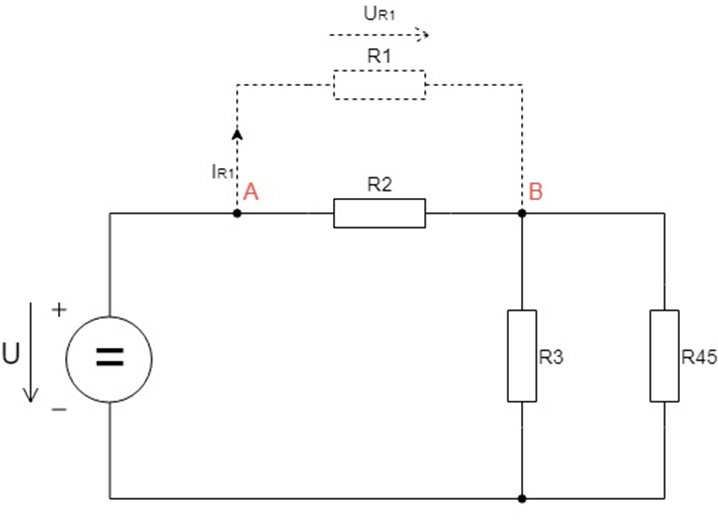
\includegraphics[width=0.6\textwidth]{fig/Pr2_1.png}
    \caption{$R_{45}~\sim~R_4,R_5$ seriove}
\end{figure}


\begin{align*}
R_{345} = \frac {R_3 \times R_{45}} {R3 + R45} = \frac {630\Omega \times 690\Omega} {630\Omega + 690\Omega} = \frac {434 700\Omega} {1320\Omega} = 329,3181\Omega
\end{align*}

\begin{figure}[H]
    \centering
    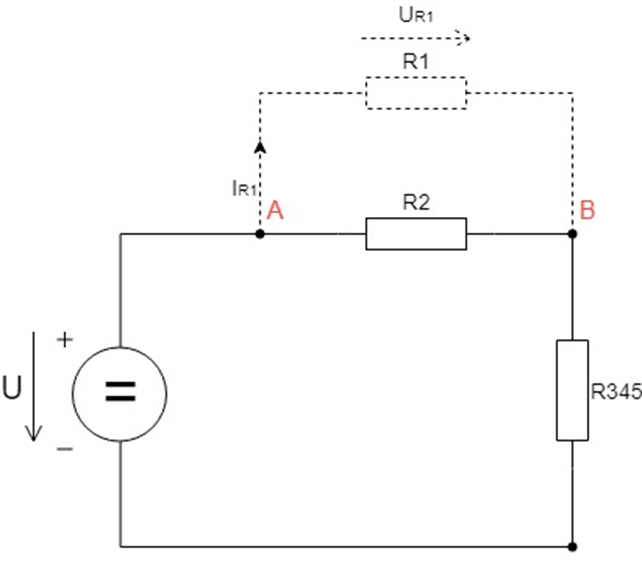
\includegraphics[width=0.6\textwidth]{fig/Pr2_2.png}
    \caption{$R_{345}~\sim~R_3,R_{45}$ parallelne}
\end{figure}
\subsection{Přechod na ekvivalentní obvod}
\begin{figure}[H]
    \centering
    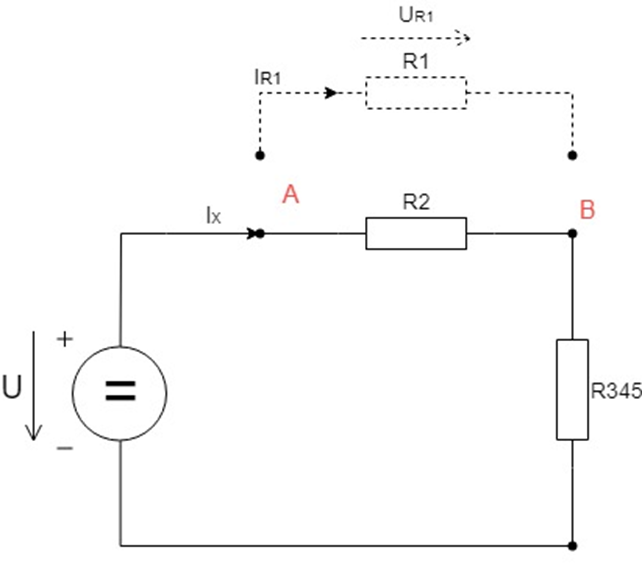
\includegraphics[width=0.6\textwidth]{fig/Pr2_3.png}
    \caption{Odpojíme větev s R1}
\end{figure}

\begin{align*}
U_i &= I_X \times R_2 + I_X \times R_{345} \textit{ (II Kir. Z.)}\\
I_X &= \frac {U} {R_2 + R_{345}} = \frac {200 V} {220\Omega + 329,3181\Omega} = \frac {200 V} {549,3181\Omega} = 0,3640 A\\
U_{AB} &= U_{R2} = I_X \times R_2 = 0,3640 A \times 220\Omega = 80,0800 V\\
R_i &= \frac {R_2 \times R_{345}} {R_2 + R_{345}} = \frac {220\Omega \times 329,3181\Omega} {220\Omega + 329,3181\Omega} = \frac {72 449,9820\Omega} {549,3181\Omega} = 131,8907\Omega\\ \\
\boldsymbol{I_{R1} }&=\boldsymbol{ \frac {U_{AB}} {R_1 + R_i} = \frac {80,0800 V} {70\Omega + 131,8907\Omega} = \frac {80,0800 V} {201,8907\Omega} = 0,3966 A}\\
\boldsymbol{U_{R1} }&=\boldsymbol{ I_{R1} \times R_1 = 0,3966 A \times 70\Omega = 27,7620 V}\\
\end{align*}

\begin{figure}[H]
    \centering
    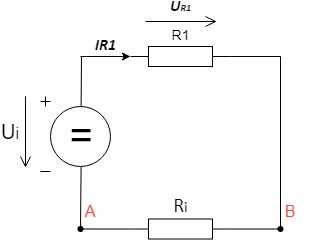
\includegraphics[width=0.4\textwidth]{fig/Pr2_4.jpg}
    \caption{Ekvivalentní obvod}
\end{figure}